\section{Materials}

paradigm is ok here, need to extend it.
From validation should be moved to results.
Should add something on psth, jpsth, correlation of time course, pca, gpfa, unitary event analysis

\myparagraph{Paradigm} 
The data comes from todo rats, trained on a grasping task that they performed while freely moving, connected to a multi-electrode device, specifically one or more tetrodes (todo which part of the cerebellum), while a high frequency camera recorded the movements, to allow marking landmarks, specifically \emph{lift}, the moment where the rat's limb was raised from the ground, \emph{cover}, when the limb was over the target, and \emph{grasp}, when the rat first touches the target. The camera frame rate was todo, so we have an uncertancy of todo on the exact time location of the landmarks.

The data has been then preprocessed and the spike sorted, so my work has been done on spike trains of neurons that could be either on the same tetrode or on a different one, allowing the distinction between neighbor and distant neurons behavior and covariance or synchrony.


\myparagraph{Environment choice} 
Working on neural data is one of the hardest challanges in the data analysis domain, since the data is often structured asymetrical, for example with different number of neurons for trials, and this requires adequate instruments to just to be able to select the data for each analysis.

To tackle this problem, I decided not to use an existing library, since one of the objectives of the work was to understand deeply how to perform efficient data analysis. 
The first problem to solve was substantially to select a given part of a spike train, giving information relative to the landmarks, the size of the resulting array, and the basic operation that I wanted to be performed on the spike train.

My language of choice for designing appropriate instruments is Julia, a new programming language developed specifically for scientific computing. My choice was guided by three main reasons: first, Julia is very fast, and since the task I needed the code to perform is for its nature the most frequent one, speed is a key factor. Second, since Julia has been built with scientific computing in mind, the code to perform the kind of operations that I needed can be very compact and elegant, which is very important for robustness and reusability of the code. The third and last reason is that Julia is a multiple dispatch programming language, which is an almost unique feature that can be exploited to write modular and reusable chunks of code, making it very elastic and easily applyable to a number of situations. This can seem very abstract, but since spike train data can take different structures, depending for example on wether we want to average over trials, use single recordings or use all the data, or if we use spike times or convoluted data, multiple dispatch is a key feature that reduces greatly the amount and complexity of code needed.

\myparagraph{Basic operations} 
The most basic operation I needed to apply on the code is convolution, either rectangular or gaussian, depending if we need to work on discrete or continuous data. Even at this most basic level, an mistake in the definition of the function can cause distortion in the data at the next stages, and can be very hard to debug. For example, when applying gaussian convolution at the limits of an array, the behavior of the convoluting function can be unexpected, and if, the extremes of the array are kept instead of feeding a bigger array to later discard them, it can cause effects such as the one in Picture1

[insert picture 1 here]

\myparagraph{Validation} 
After I built the preprocessing steps, I validated them on the previous analyses already performed, the first being Peri-Stimulus Time Histogram (PSTH). PSTH shows graphically the neurons that are more active when the subject is stimulated, or in the case of this experiment, when it spontanously moves his arm. It is useful to assest the actual correlation between the action and the neural activity, which is usually normalized, so that one can properly distinguish abnormal activity without being confused by neurons that are naturally more active than others.

The spiketrains used to produce the PSTH come from the recordings of all neurons 5 seconds before and after the \emph{lift} landmark. They have been averaged by trials, and convolved with a $\sigma=10$ gaussian kernel, and normalized using the firing rates between 5 and 3 seconds before the landmark. To give an example of the framework built to deal on the data, this is the code used to generate the data:
\begin{lstlisting}[frame=single]
spiketrains = slice(data.t, data.lift, around=[-5000, 5000], 
		    convolution=true, normalization=true, 
		    average=true, over=[-5000, -2000])
\end{lstlisting}
\begin{figure}[h]
	\centering
	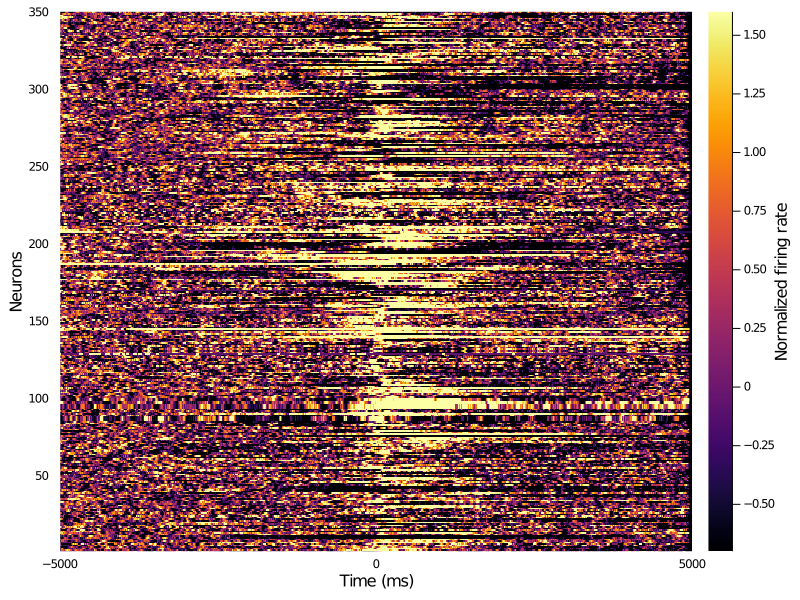
\includegraphics[scale=0.5]{../../plots/psth.pdf}
	\caption{Normalized peri-event histogram}
	\label{fig:psth}
\end{figure}


After PSTH, I performed one more analysis, to be also validate that convolution was working properly. It consisted in calculating the correlation coefficient of the convoluted signals of neighbor vs distant neurons around landmarks, and you can see the results in picture 3.

\begin{figure}[h]
	\centering
	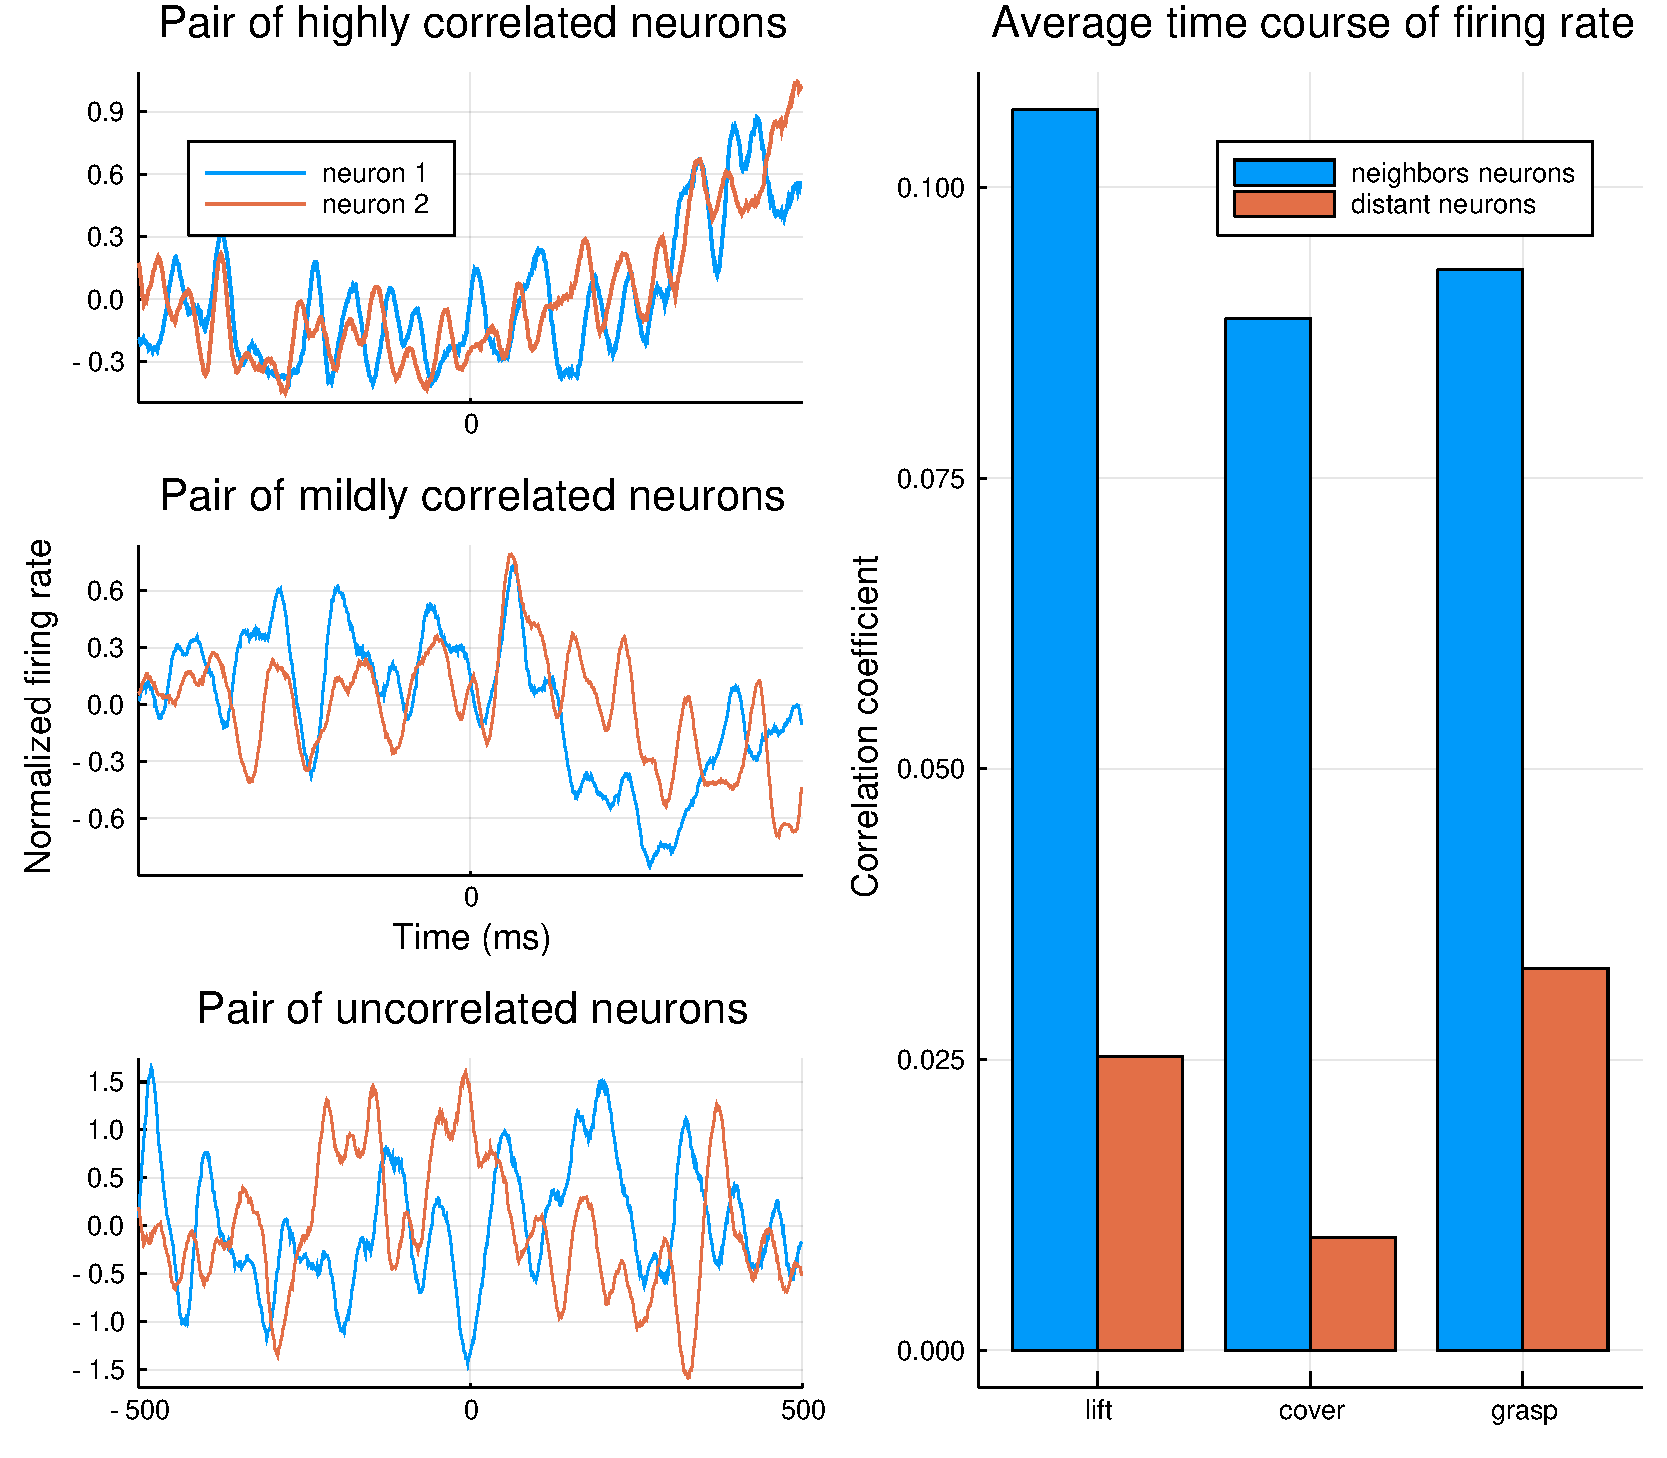
\includegraphics[scale=0.5]{../../plots/corr-coef.pdf}
	\caption{Firing time course around lift for pairs of neighbouring cells and correlation of average time course firing rate of neighbour vs distant nerons}
	\label{fig:corr-coeff}
\end{figure}

\myparagraph{Dynamics} 
The analyses that I performed are mostly focused on characterizing the dynamics shown by neural signals while the animal is performing a task. 

The study of the dynamics is aimed at understanding the algorithmic level of Marr, and has the potential to give insights on which operations recurrent neural networks in the brain are performing. The knowledge of those operation is in turn precious for developing artificial systems with comparable computational capabilities, and in fact it has been proposed by Hassabis [cit] that neuroscience should focus on researching the computational and algorithmical levels. 

Altough Computational Neuroscience research is undoubtely very useful for advances in Machine Learning, that is not its only purpose, so in the continuation of this work I intend to perform some validation on simulated data, aiming to obtain insight on the implementation level, that is how the computations performed can be carried on by (simulated) biological neurons.

There are many possible approaches to tackle the study of dynamics, and I decided to start from the most simple ones and then move towards more complex methods.

\myparagraph{Dimensionality reduction}
Since the advent of multi-electrode recordings and optical imagining has begun, neuroscience has started looking for proper method to analyse the huge amount of data resulting from state of the art recording methods.
One key approach has been dimensionality reduction techniques, which are extensively use to explore neural data and analyse neural dynamics through the observation of trajectories.
The most simple dymensionality reduction technique is Principal Component Analysis (PCA) , which has the advantage of being very interpretable, since it only applies linear transformation to the data to find the projection in a lower dimensional plane which maximize the variance in the data.

Unfortunately, PCA also has disadvantages, for example it is very easily confounded by a number of factors - for example very active neurons - so it is good pratice to average trials and normalize the data.

